\documentclass{article}

\usepackage[ngerman]{babel}
\usepackage{pdfpages}
\usepackage{amssymb}
\usepackage{amsmath}
\usepackage{mathtools}
\usepackage{graphics}
\usepackage{graphicx}
\usepackage{geometry}
\usepackage{float}

\geometry{
 a4paper,
 total={170mm,257mm},
 left=25mm,
 top=25mm,
}


\begin{document}

\thispagestyle{empty}
\vspace*{\fill}
\begin{center}
	\Huge
	\textbf{Universit"at zu K"oln}\\
	\LARGE
	\textbf{Institut für Astrophysik}\\
	\vspace{2cm}
	\textbf{Versuchsprotokoll}\\
	\vspace{0.5cm}
	\large
	\textbf{B1.1: Infrarotabsortption in $CO_2$}\\
	\normalsize
	\vspace{2cm}
	\begin{tabular}{r l}
		Autoren: 	& Jesco Talies$^1$\\
					& Timon Danowski$^2$\\
                    & Erik Gaßmus$^3$\\
		Durchgefuehrt am:	& 8.02.2021\\
		Betreuer:	& Bettina Heyne
	\end{tabular}
\end{center}
\vfill\footnotesize
$^1$ jtalies@smail.uni-koeln.de, Matrikel-Nr.: 7348338\\
$^2$ tdanowsk@smail.uni-koeln.de, Matrikel-Nr.: 7348629\\
$^3$ e.gassmus@gmail.com, Matrikel-Nr.: 7329899
\normalsize

\newpage
\thispagestyle{empty}
\tableofcontents
\clearpage
\setcounter{page}{1}
\section{Einleitung}
    In diesem Versuch soll der Zusammenhang zwischen dem quantenmechanischen Phänomen der Photonenabsorption
    in Gasen und den daraus folgenden makroskopischen Erscheinungen wie z.B. dem Treibhauseffekt untersucht werden.
\section{Theoretische Vorbereitung}
    \subsection{Elektromagnetisches Spektrum}
        Das Elektromagnetische Spektrum beschreibt die gesamte Breite der elektromagnetischen Wellen, das bedeutet
        von Ultra-Langwellen mit einer Wellenlänge von etwa $10^7$m bis hin zu Gammastrahlung mit etwa $10^{-11}$m. Dabei
        bescheibt nur ein kleiner Ausschnitt um $\lambda=500\cdot 10^{-9}m=500nm$ das für uns sichtbare Licht und den daran 
        angrenzenden Infrarotbereich mit etwa $\lambda=10^{-6}m=1\mu m$.\\
        Eine wichtige Formel im Zusammenhang mit dem elektromagnetischen Spektrum beschreibt die Umrechnung der Wellenlänge
        $\lambda$ in eine Frequenz $\nu$.
        \begin{equation}
            \nu = \frac{c}{\lambda}
        \end{equation}
        wobei c die Lichtgeschwindigkeit bezeichnet.
        \begin{figure}[H]
            \centering
            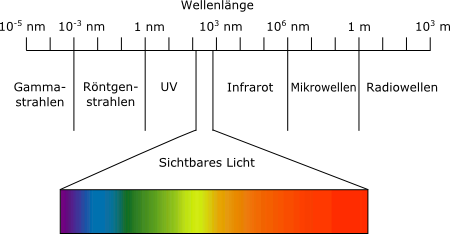
\includegraphics{Images/EMSpektrum.png}
            \caption{Abbildung des Elektromagnetischen Spektrums}
        \end{figure}
        \begin{center}
            Quelle\footnote{http://www.physicoro.de/umrechnungen/spektrum.php?lg=de}
        \end{center} 
        
    
    \subsection{Planck'sche Strahlungsformel}
        Die Planck'sche Strahlungsformel beschreibt die spektrale Energiedichte der Strahlung eines 
        Schwarzkörpers als Funktion der Wellenlänge und Temperatur. Das Planksche Strahlungsgesetzt als Ganzes
        gibt dann für jede Temperatur die Verteilung der Schwarzkörperstrahlung in Abhängigkeit der Wellenlänge der
        Strahlung an.\\
        Die Planck'sche Strahlungsformel lautet
        \begin{equation}
            M_{\lambda}(\lambda,T) = \frac{2\pi hc^2}{\lambda^5}\frac{1}{e^{\frac{hc}{\lambda kT}}-1}dAd\lambda
        \end{equation}
        Woraus sich folgende Verteilungen ergeben
        \begin{figure}[H]
            \centering
            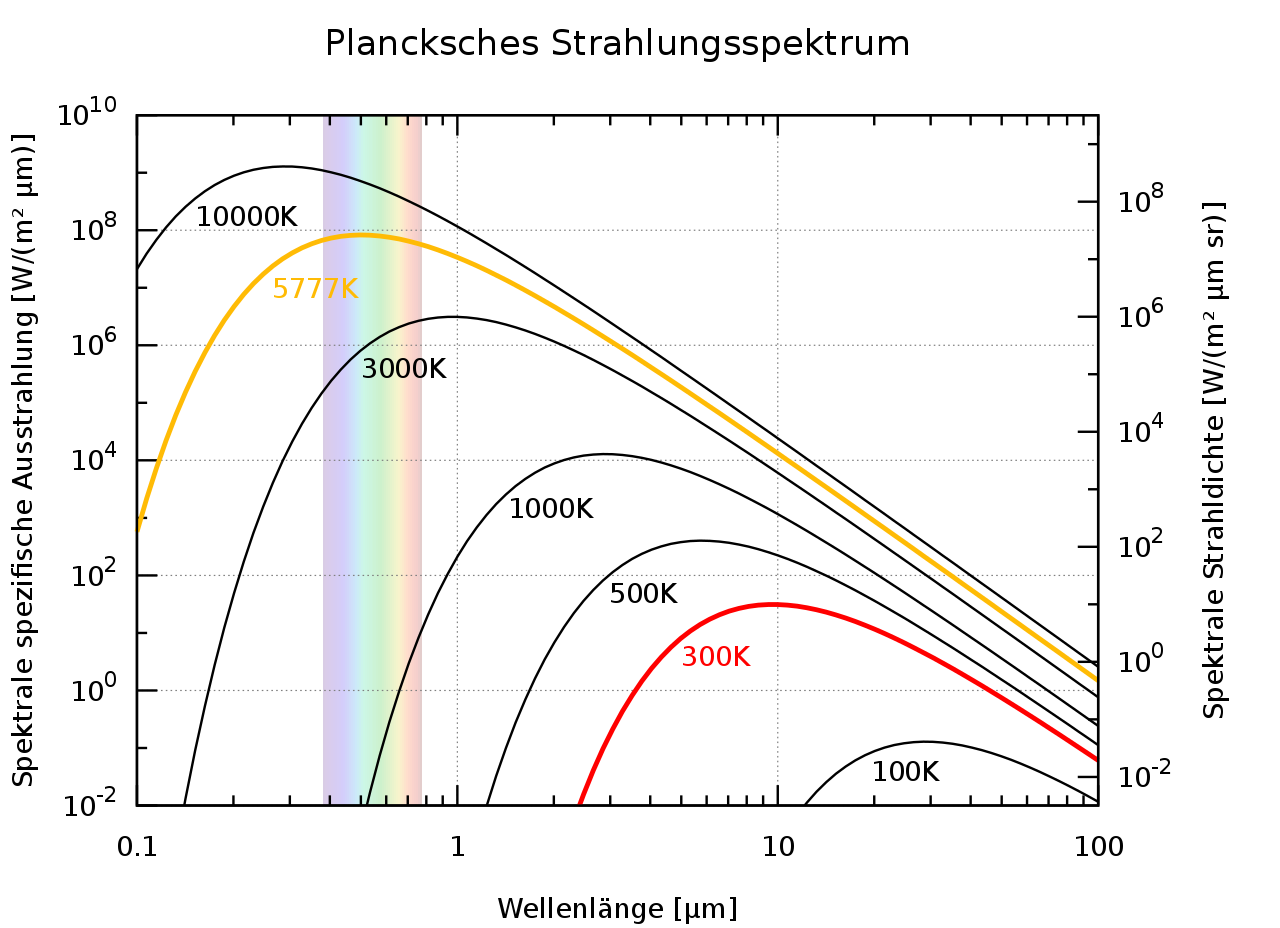
\includegraphics[width=0.9\textwidth]{Images/PlanckStrahlung.png}
            \caption{Planksches Strahlungsspektrum}
        \end{figure}
        \begin{center}
            Quelle\footnote{https://de.wikipedia.org/wiki/Datei:BlackbodySpectrum\_loglog\_de.svg}
        \end{center}
        Wie auch der Abbildung bereits zu erkennen ist, verschiebt sich die Lage des Maxmimums bei steigenden
        Temperaturen in Richtung von kleineren Wellenlängen. Diese Verschiebung lässt sich über das Wiensche Strahlungsgesetzt
        bestimmen.
        \begin{equation}
            \lambda_{Max} = \frac{2897,8 \mu mK}{T}
        \end{equation}


    \subsection{Elektrisches Dipolmoment}
        Das elektrische Dipolmoment beschreibt eine räumliche Ladungstrennung, d.h. die verschiedenen Vorzeichen
        der Ladungen zweier Teilchen eines Körpers. Liegt der Schwerpunkt der Gesamtladung der Elektronen nicht auf dem der Protonen,
        so besitzt der Körper ein Elektrisches Dipolmoment.\\
        Dieses Dipolmoment $\vec{p}$ lässt sich Bestimmen über
        \begin{equation}
            \vec{p} = q \cdot l \cdot \vec{e_l}
        \end{equation}
        mit l als skalarem Abstand der Ladungen und $\vec{e_l}$ dessen Richtung.\\
        Integriert man über einen Körper mit mehreren solcher Momente erhält man das gesamte Dipolmoment über
        \begin{equation}
            \vec{p} = \int_V \rho(\vec{r})\cdot\vec{r}d^3r
        \end{equation}
         \\
        Damit eine Wechselwirkung mit einem Photon stattfinden kann, muss sich das Dipolmoment beim Übergang ändern,
        da durch Anregung eine Ladungsumverteilung stattfindet. Damit ein Molekül nun wechselwirken kann, muss es mindestens
        mit der Frequenz des Interagierenden Photons schwingen. Dieses Dipolmoment ist jedoch lediglich während des Übergangsvorhanden,
        und wird als Übergangdipolmoment bezeichnet.
        \begin{equation}
            \mu_{EA} = \int \psi_E^* \vec{\mu} \psi_A dr
        \end{equation}
        Dabei beschreiben $\psi_E$ und $\psi_A$ die Wellenfunktion der beiden Zustände und $\vec{\mu}$ den Operator
        des El. Dipolmoments.

    \subsection{Freiheitsgrade}
        Die Freiheitsgrade f beschreiben die Anzahl der Unhabhängigen Bewegungsmöglichkeiten durch die Energie
        aufgenommen werden kann. Jedes Molekül mit N atomen hat 
        $$ f = 3n $$
        Freiheitsgrade, da man die Position des Atoms genau über 3 Koordinaten definieren kann.
        Diese Freiheitsgrade lassen sich aufteilen in Translation, Rotation und Schwingungen.
        \begin{equation}
            f = f_{trans} + f_{rot} + f_{vib}
            \Rightarrow f_{vib} = 3n - f_{trans} - f_{rot}
        \end{equation}
        Für N-Atomige Moleküle gilt:\\
        $f_{trans} = 3$ (3D-Translation)\\
        $f_{rot} = 2$(bzw.$3$) Da bei Linearen Molekülen die Rotation um die Z-Achse kein Trägheitsmoment wirkt, kann diese auch keine Energie aufnehmen.\\
        $f_{vib} = 3n-f_{trans} - f_{rot}$\\
    
    \subsection{Normalschwingungen}
        Der Begriff Normalschwingung dient als Überbegriff für die verschiedenen Schwingungsarten eines Moleküls.
        Die $3n-f_{trans} - f_{rot}$ lassen sich aufteilen in
        \begin{enumerate}
            \item Valenzschwingungen (Schwingungen entlang der Bindungsachsen)
            \item Deformationsschwingungen (Schwingungen unter Deformation der Bindungen)
        \end{enumerate}
        Das 3 Atomige $CO_2$ Molekül ist linear, woraus 
        $$ 3\cdot 3 - 3 - 2 = 4$$
        Normalschwingungen Folgen. Die Antisymetrische und Symetrische Valenzschwingung ($v_{as}, v_s$) und den
        Deformationsschwingungen parallel und senkrecht zur Zeichenebene.
        \begin{figure}
            \centering
            \includegraphics{Images/molekülschwingungen.jpeg}
            \caption{Molekülschwingungen}
            %https://www.google.com/url?sa=i&url=http%3A%2F%2Fphysik.uni-graz.at%2F~pep%2FLehre%2FAMFP%2Flecture06.pdf&psig=AOvVaw1s-ljtqjA7wKrdMSBywd86&ust=1616190013489000&source=images&cd=vfe&ved=0CAIQjRxqFwoTCPje5ZHnuu8CFQAAAAAdAAAAABAD
        \end{figure}
    
    \subsection{Zweiatomiges Molekül}
        \subsubsection{Energieniveaus}
            Für die kinetische Energie eines Starren Rotors ergibt sich 
            \begin{equation}
                E_{rot} = \frac{\hbar^2 J(J+1)}{2I}
            \end{equation}
            mit J als Gesamtdrehimpuls und I als Trägheitsmoment. Daraus ergeben sich für verschiedene
            Gesamtdrehimpulse die verschiedenen Energieniveaus.
        \subsubsection{Rotationsanregung}
            Für die Rotationsenergie erhält man klassisch
            \begin{equation}
                E_{rot} = \frac{1}{2}I\omega^2=\frac{1}{2}\frac{\vert J\vert^2}{I}
            \end{equation}
            Mit I=MR.\\
            Dabei ist $R_e$ der Gleichgewichtsabstand, $B_e$ die Rotationskonstante und $\omega_e$ die Schwingungsfrequemz.
        \subsubsection{Vibrationsanregung}
            Für die Vibrationsenergie Ergibt ich mit der Vibrationsquantenzahl $v=0,1,2,3..$
            \begin{equation}
                E_{vib} = (v + \frac{1}{2})\hbar \omega
            \end{equation}
        \subsubsection{Vergleich}
            Die Energien zur Anregung von Vibrationsübergängen liegen typischerweise im Infraroten (~$10^5$nm)
            wohingegen Rotationsübergänge bereits im submm Bereich angeregt werden können.
    
    \subsection{IR-Aktivität}
        Bei der Bestrahlung von $CO_2$ mit em Wellen werden bestimmte  Frequenzbereich absorbiert, in diesem Fall
        Infrarotstrahlung, da diese im Bereich des Rotationsvibrationsniveaus von $CO_2$ liegt. Die Absorbierte IR-Strahlung
        regt Schwingungen an, welche in Form von Ausschlägen im Spektrum sichtbar werden.\\
        Da Wechselwirkungen zwischen em-Strahlung und Molekülen nur dann auftreten kann, wenn dieses ein veränderbares
        oder ein induziertes Dipolmoment aufweist, sind nicht alle Normalschwingungen von $CO_2$ IR-Aktiv.
        Es sind lediglich die Antisysmetrische Valenzschwingung und die Deformationsschwingungen IR-Aktiv.
    
    \subsection{IR-Spektrum von $CO_2$}
        Das IR-Spektrum von $CO_2$ bei niedrigem Druck sieht folgendermaßen aus
        \begin{figure}[H]
            \centering
            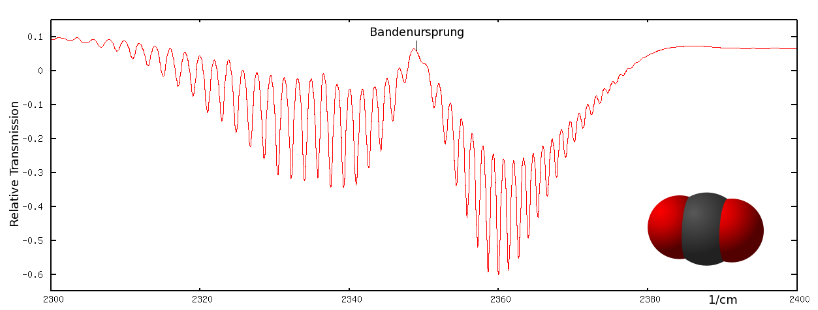
\includegraphics[width=0.9\textwidth]{Images/IRSpektrum.PNG}
            \caption{FTIR-Spektrum von $CO_2$ bei geringem Druck}
        \end{figure}
        Erhöht man den Druck in dem Messaufbau, stellt man eine Linienverbreiterung proportional zur
        Druckänderung fest. Bis zu Drücken von 10mbar ist diese Verbreiterung linear, danach verschiebt sich
        das Spektrum zu höheren Frequenzen und wird Asymetrisch.

    \subsection{Rotationsbande}
        Die Wechselwirkung zwischen einer em-Welle und einem Molekül, wird durch die Multipolmomente u.a. dem Dipolmoment ermöglicht. 
		Für Übergänge in andere Zustände gibt es Auswahlregeln, so dass manche Übergänge \textit{verboten} sind.
		Für Vibrations- und Rotationsübergänge sind diese:
		\begin{equation}
			\Delta \nu = \pm1
		\end{equation}
		\begin{equation}		  
			\Delta J = \pm1
		\end{equation}		   	
    	
    	Da Übergänge mit $\Delta \nu = -1$ im Infraroten keine Rolle spielen, wird im folgenden nur $\Delta \nu = +1$ betrachtet.
    	Übergänge mit $\Delta J = +1$ führen zu einer positiven Frequenzverschiebung im Bezug auf die Frequenz $\nu_0$ des reinen Vibrationsübergangs (R-Zweig), $\Delta J = -1$ zu einer negativen (P-Zweig)
    
    \subsection{Photonen}
        Ein Photon mit der Frequenz $\nu$ transportiert die Energie
        \begin{equation}
            E = h\cdot \nu
        \end{equation}
        Dies entspricht einer Wellenlänge
        \begin{equation}
            \lambda = \frac{h\cdot c}{E}
        \end{equation}
        und einer Wellenzahl von
        \begin{equation}
            \vec{\nu} = \frac{1}{\lambda} = \frac{E}{h\cdot c}
        \end{equation}
    
    \subsection{Gaußsche Normalverteilung}
        Die Gaußverteilung ist eine kontinuierliche Verteilung, ihre Wahrscheinlichkeitsdichte ist
        gegeben durch
        $$ P(x,\mu, \sigma) = \frac{1}{\sigma\sqrt{2\pi}}\cdot e^{-\frac{1}{2}(\frac{(x-\mu)^2}{\sigma})}$$
        Dabei ist $\mu$ der Mittelwert und $\sigma^2$ die Varianz.
    
    \subsection{Teppenfunktionen}
        Sei $[a,b] \subset \Re $ ein geschlossenes Intervall und $\tau:[a,b]\rightarrow\Re$ eine Funktion
        auf diesem Intervall.Dann heißt $\tau$ Treppenfunktion, falls eine Unterteilung
        $a=x_0<x_1<...<x_n=b$ existiert, so dass $\tau|(x_i-1,x_i)=const. \forall i\in [1,n]$ Wir bezeichnen die Menge aller
        Treppenfunktionen auf dem Intervall [a,b]mit T[a,b].
        Das Integral einer Treppenfunktion sieht
        folgendermaßen aus:
        \begin{equation}
            \int_a^b \tau(x)dx:=\sum_{i=1}^n c_i\cdot (x_i-x_i-1)n_i=1
        \end{equation}
        Man kann die Treppenfunktion nutzen um das Integral von glatten Funktionen anzunähern.
        Gehen wir nun davon aus, dass die Abstände zwischen den Punkten [$x_i,x_i+1$] konstant sind 
        für alle $i\in[1,n]$. Wir  bleiben  dabei  dass $x_0=a$ und $x_n=b$, dann kann man den Abstand
        zwischen den Punkten schreiben als:$h=\frac{b-a}{n}$. Für $c_i$ nehmen wir immer
        den jeweiligen Funktionswert $f(x_i)=f(a+ih)$. Damit können wir für eine beliebige glatte Funktion
        (die im Intervall [a,n] nicht null wird) sagen:
        \begin{equation}
            \int_a^b f(x)dx\approx h\cdot\sum_{i=1}^n f(x+ih)=0
        \end{equation}
        Zu Beachten ist jedoch,
        dass die Annäherung eines Integrals durch eine Treppenfunktion eine ungenaue Methode ist.
        Mit ähnlich großem Aufwand lässt sich ein Integral genauer berechnen, nämlich über die Trapeze.
    
    \subsection{Gewichteter Mittelwert}
        Der gewichtete Mittelwert unterscheidet sich kaum vom normalen Mittelwert. Beim gewichteten Mittelwert
        einer Messgröße X wird jeder Messwert $x_i$ mit einer Gewichtung $w_i$ multipliziert. Anschließend wird durch
        die Summe der Gewichtungen geteilt um den Wert wieder zu normieren.
        \begin{equation}
            \bar{x} = \frac{1}{\sum_{i}w_i}\cdot \sum_{i} x_i\cdot w_i
        \end{equation}
        Die Gewichtungsfunktion muss passend gewählt werden. Eine mögliche Wahl die vom Fehler $\Delta x_i$
        wäre zum Beispiel 
        \begin{equation}
            w_i = \frac{1}{\sqrt{\Delta x_i}}
        \end{equation}

    \subsection{Lambert-Beer-Gesetz}
        Das Lambert-Beersche Gesetz beschreibt die Abschwächung der Intensität einer Strahlung mit Wellenlänge
        $\lambda$ bei Transmission durch eine absorbierende Substanz.
        \begin{equation}
            E_{\lambda} = log_{10}(\frac{I_0}{I_1}) = \epsilon_{\lambda} \cdot c \cdot d
        \end{equation}
        Der Absorptionskoeffizient ist in unserem Fall die einzig explizit frequenzabhängige Größe. Bei Drücken
        von etwa 1bar kann beobachtet werden, dass das Spektrum sich einer Gaußkurve nähert.\\
        Da $E \propto \epsilon(\nu)$ kann davon ausgegangen werden, dass wir den Absorptionskoeffizienten 
        $$\epsilon(\nu) = \beta exp(-\frac{(\nu - \nu_0)^2}{2\sigma^2})$$
        (mit $\beta$ als Proportionalitätskonstante und $\sigma$ als Breite der Gaußverteilung) als Gaußkurve ausdrücken
        können. Daraus folgt die Transmission
        \begin{equation}
            g_s(\nu) = \frac{I(\nu)}{I_0} = exp(-\epsilon(\nu)\cdot cd) = exp(-cd\beta\cdot e^{\frac{(\nu-\nu_0)^2}{2\sigma^2}})
        \end{equation}
    
    \subsection{Atmosphärischer Treibhauseffekt}
        Die Photosphäre der Sonne strahlt mit einer Temperatur von etwa 6000~K bei einem Strahlungsmaximum
        von etwa 500~nm. Von der Erde aus, kann man diese Temperatur über das Stefan-Boltzman Gesetz bestimmen, bei
        dem die abgestrahlte Leistung pro Fläche proportional zu $T^4$ ist.\\
        Strahlung in diesem Spektralbereich kommt beinahe ungehindert durch unsere Atmosphäre. Dadurch erwärmt
        sich die Erdoberfläche auf etwa 300~K. Die Erdoberfläche emitiert daraufhin Strahlung gemäß des Wienschen Verschiebungsgesetzes
        im 500~nm Bereich. Diese Strahlung wird von den Treibhausgasen, unter anderem $CO_2$, absorbiert, welches zurzeit
        etwa 0.04~\% der Erdatmosphäre ausmacht.\\
        Da gute Absorber nach dem Kirchhofschen Strahlungsgesetzt auch gute Emitter sind, geben diese Gase die 
        absorbierte Infrarotstrahlung wieder an die Oberfläche ab.\\
        Ohne den oben beschriebenen Effekt würde sich die Erde bei einer Oberflächentemperatur im globalen Mittel von
        etwa -18~°C im Gleichgewicht mit dem umliegenden Weltall befinden, da die Temperatur im Mittel jedoch +14~°C
        beträgt, schreibt man die 32~°C Unterschied dem Treibhauseffekt zu.
    \section{Versuchsaufbau}
        Der Aufbau besteht aus einer breitbandigen IR-Quelle, einer Absorbtionszelle die nach bedarf mit verschiedenen
        Konzentrationen von $CO_2$ befüllt werden kann und einem breitbandigen IR-Detektor.
        Die IR-Quelle wird dabei durch eine Wendel aus Metalldraht als Schwarzkörper genähert um ein möglichst breites
        Spektrum zu erzeugen.\\
        Die Temperatur des Gases in der Absorptionszelle ist während des ganzen Versuchs über das Thermometer beobachtbar.\\
        Bei unserem Detektor handelt es sich um einen pyroelektrischen Detektor, das Kristallgitter eines solchen
        pyroelektrischen Materials wird bei Absorption eines IR-Photons lokal verformt, sodass sich die Abstände
        zwischen positiven und negativen Ionen ändern und eine messbare Spannung abfällt.
        Diese Spannung wird an einen X-Y-Plotter weitergegeben, wodurch man den Ort der maximalen Intensität ermitteln kann.
        \begin{figure}[H]
            \centering
            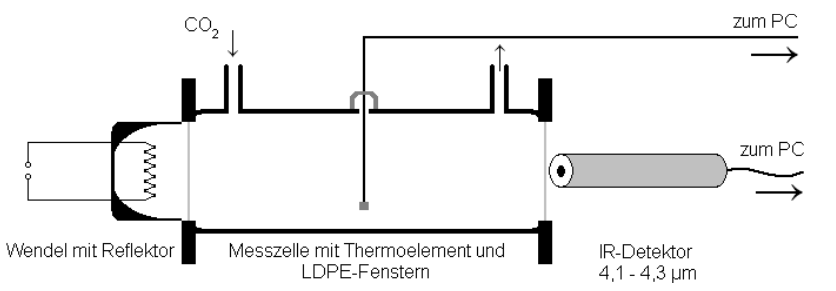
\includegraphics[width=0.9\textwidth]{Images/Versuchsaufbau.PNG}
            \caption{Versuchsaufbau}
        \end{figure}
    %\section{Durchführung}

    \section{Auswertung}
        \subsection{Zeitkonstante der IR-Quelle und Drifteffekte}
            Um in den folgenden Abschnitten weiter mit den Messdaten zu arbeiten müssen diese zunächst von dem Einfluss der Drifteffekte
            befreit werden. Dazu müssen diese Effekte zunächst bestimmt werden.
            Dazu lässt sich die Messkurve in 3 Abschnitte linearen Anstiegs unterteilen:
            \begin{figure}[H]
                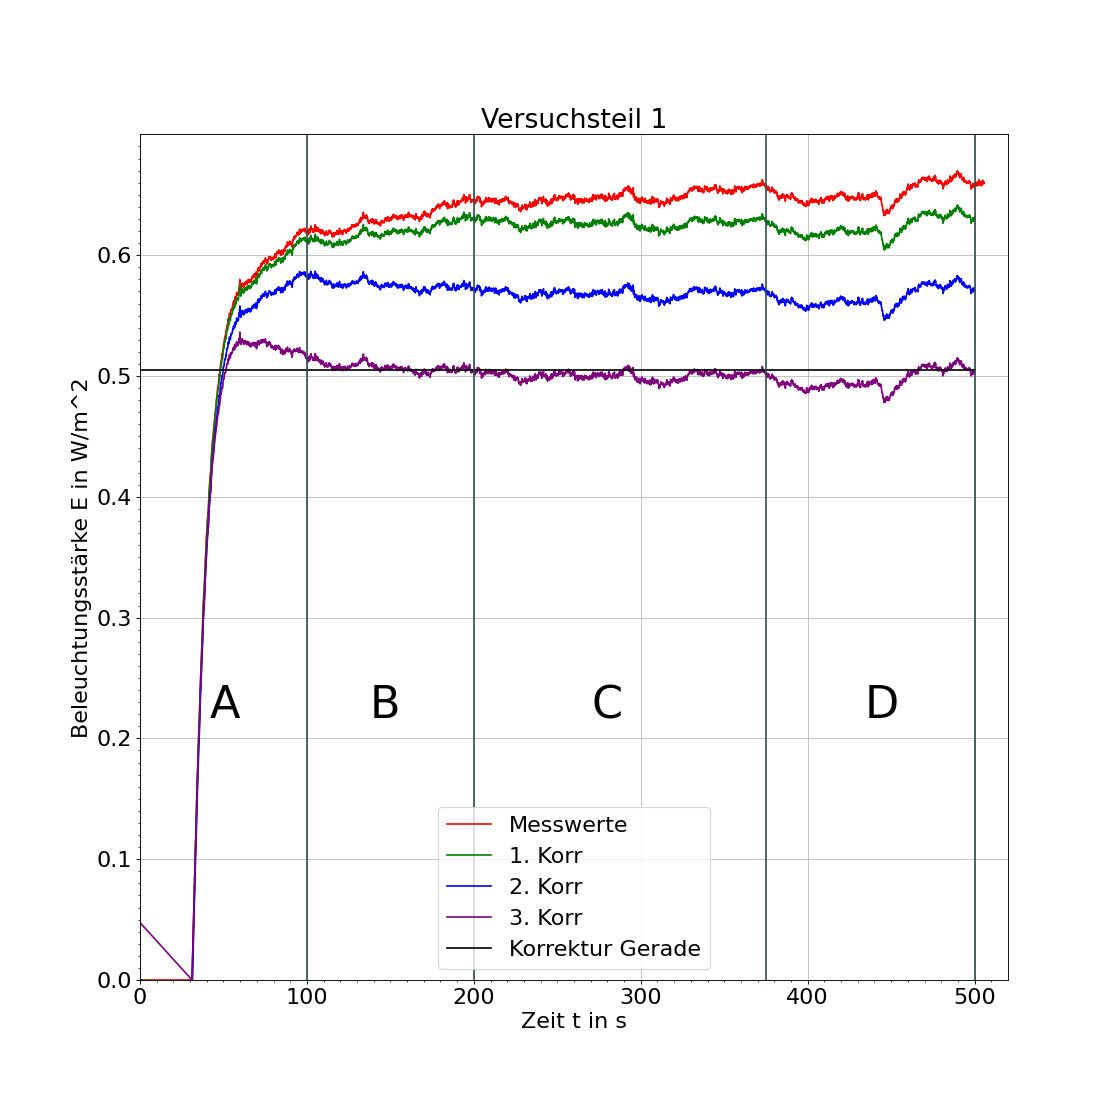
\includegraphics[width=0.9\textwidth]{Daten/DriftKorrektur.png}
                \label{DriftKorr}
                \caption{Driftkorrektur}
            \end{figure}
            Dabei sind unsere Intervalle:
            \begin{equation}
                I_1 = [70,100], I_2=[100,200],I_3=[200,375]
            \end{equation}
            In diesen Intervallen lässt sich nur über eine Regressionsgerade die Steigung ermitteln.
            Aus diesen Steigungen ergeben sich dann folgende Korrekturfunktionen mit denen
            die Drifteinflüsse, durch Subtraktion, herausgerechnet werden können.
            \begin{equation}
                g_1(t)=
                \begin{cases}
                    m_1\cdot t, 0<t<t_1\\
                    g_1(t_1),t\geq t_1
                \end{cases}
                = 
                \begin{cases}
                    7.56e-5\cdot t, 0<t<375\\
                    0.028,t\geq 375
                \end{cases}
            \end{equation}
            
            \begin{equation}
                g_2(t)=
                \begin{cases}
                    m_2\cdot t, 0<t<t_2\\
                    g_2(t_2),t\geq t_2
                \end{cases}
                = 
                \begin{cases}
                    2.91e-5\cdot t, 0<t<200\\
                    0.058,t\geq 200
                \end{cases}
            \end{equation}

            \begin{equation}
                g_3(t)=
                \begin{cases}
                    m_3\cdot t + b_3, 0<t<t_3\\
                    g_3(t_3),t\geq t_3
                \end{cases}
                = 
                \begin{cases}
                    1.16e-4\cdot t+0.0475, 0<t<100\\
                    0.116+0.0475,t\geq 100
                \end{cases}
            \end{equation}
            Durch Subtraktion der Korrekturfunktionen ergeben sich die Korrekturkurven wie in
            \ref{DriftKorr} eingezeichnet. In der letzten Korrektur wird zudem der Ordinatenwert
            der Regressionsgeraden von $b_3=0.0475$ addiert um die Geraden auf den Nullpunkt bei
            Steigungsbeginn zu eichen. \\
            Diese eben bestimmten Drifteffekte lassen sich bei diesem Versuchsaufbau auf eine Auswahl
            verschiedener Ursachen zurückführen, so führt das erhitzen der verschiedenen Elektronischen
            Komponente wie Kabel, auch wenn hier kaum feststellbare Änderungen auftreten sollten, oder
            Spulen, insbesondere die Heizspule zu einer Änderung des elektrischen Widerstands wodurch
            sich der Energiefluss verändert und damit die Intensität. Durch die notwendige
            IR-Strahlung der Heizspule kommt es zusätzlich zur Erwärmung der Umgebung und des Detektors,
            sodass sich auch in der Luft und ggf. auch im Detektor die Materialeigenschaften ändern.
            Betrachtet man den Lauf der Energie und die Stärke und Dauer der Drifteffekte wären die Wahrscheinlichsten Ursachen:
            $$ A\rightarrow \text{Erwärmung der Wendel und Änderung der El. Eigenschaften}$$
            $$ B\rightarrow \text{Erwärmung der Luft durch die IR-Strahlung}$$
            $$ C\rightarrow \text{Änderung der El. Eigenschaften des Detektors}$$
            Betrachtet man nun nach der Korrektur der Messwerte die durch die Korrektur entstandene Abweichung
            so zeigt sich für folgende drei exemplarische Zeitpunkte eine relative Abweichung.
            \begin{equation}
                Rel.Abw. = \frac{E(t)-E_{korr}(t)}{E(t)}
            \end{equation}
            \begin{center}
                \begin{tabular}{|c|c|}
                    \hline
                    Zeit [s] & Relative Abweichung [\%] \\
                    \hline
                    100 & 16,95 \\
                    200 & 21,94 \\
                    300 & 23,06 \\
                    \hline
                \end{tabular}
            \end{center}
            Diese entstandenen Abweichungen wirft die Frage nach der Messgenauigkeit unserer 
            korrigierten Kurve auf. Um zu Ermitteln ab wann die Abweichung der Messung von dem
            endgültigen, stationären Wert bei $t>t_1$ unter 3\% liegt, wurde die Abweichung des
            Mittelwerts von je 10s Messzeit von dem Mittelwert des stationären Bereichs untersucht:
            \begin{equation}
                \begin{aligned}
                    I = \frac{1}{100}\cdot \sum_t^{t+10s}{E(i)} \\
                    I_0 = \frac{1}{t_{max}-t_1}\cdot \sum_{t_1}^{t_{max}}{E(i)}\\
                    \Delta I = 1-\frac{|I-I_0|}{I_0} \\
                \end{aligned} 
            \end{equation}
            \begin{center}
                \begin{tabular}{|c|c|c|c|c|}
                    \hline
                    Startzeit [s] & $I[\frac{W}{m^2}]$ & $I_0[\frac{W}{m^2}]$ & $\Delta I[\%] $ \\
                    \hline
                    0   & 0,032 & 0,497 & 6,5 \\
                    30  & 0,356 & 0,497 & 72,0 \\
                    70  & 0,522 & 0,497 & 94,9 \\
                    80  & 0,520 & 0,497 & 95,2 \\
                    90  & 0,514 & 0,497 & 96,59 \\
                    100 & 0,509 & 0,497 & 97,53 \\
                    110 & 0,506 & 0,497 & 98,17 \\
                    120 & 0,509 & 0,497 & 97,47 \\
                    130 & 0,509 & 0,497 & 97,59 \\
                    ... & ...   &  ...  & ... \\
                    330 & 0,502 & 0,497 & 98,82 \\
                    340 & 0,501 & 0,497 & 99,17 \\
                    350 & 0,500 & 0,497 & 99,43 \\
                    \hline 
                \end{tabular}
            \end{center}
            Dieser Tabellenausschnitt zeigt, dass ab ca. 100s die Genauigkeit über 97\% liegt, wobei die Letzten
            Einträge demonstrieren, dass es auch im stationären Bereich noch zu geringfügigen statistischen
            Schwankungen kommt.\\
            Nun zur eigentlichen Auswertung, die Anpassung von
            \begin{equation}
                f(t) = c\cdot(1-exp(\frac{-t}{\tau}))
            \end{equation}
            an die Messpunkte. Dabei ist c bereits bekannt, als Maximalwert, an die sich die e-Funktion
            asymptotisch nähert. Dieser ist bereits aus der Tabelle abzulesen und ist hier $c=0,497[\frac{W}{m^2}]$.
            Der freie Parameter $\tau$ hingegen ist durch Anpassung zu bestimmen. Dafür sollte zunächst ein
            passendes Zeitintervall gewählt werden, um ein möglichst präzises Ergebnis zu erhalten.
            Dafür wurde zunächst der durch die Verschiebung erzeugte Nullstelle ermittelt woraus das Intervall
            $$ t \in [31.2s,500s]$$ 
            gewählt wurde. Verschiebt man nun die Zeiten um 31,2 Sekunden um die Nullstelle in den Ursprung
            zu legen, erhält man folgenden Fit:
            \begin{figure}[H]
                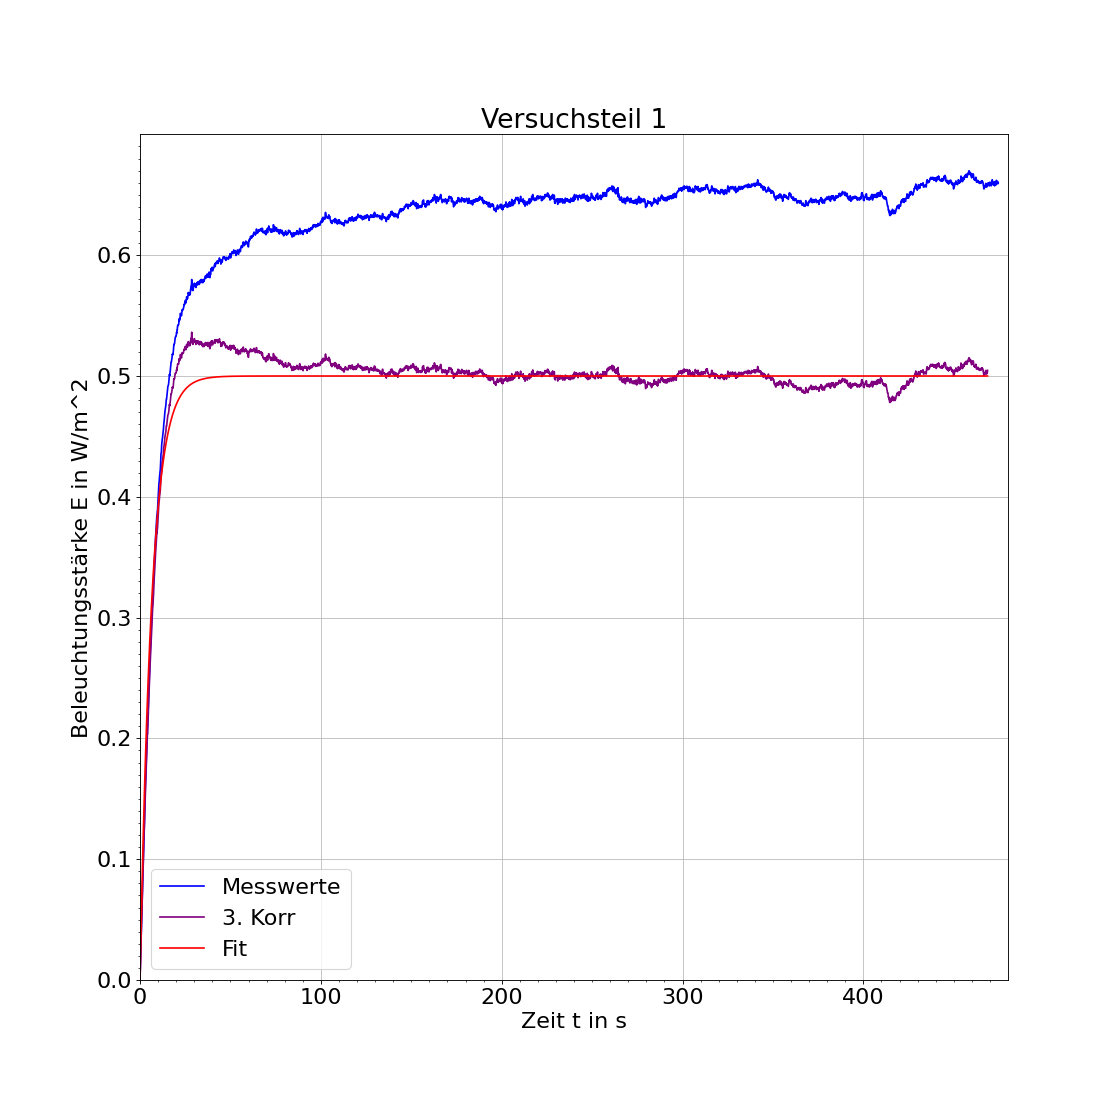
\includegraphics[width=0.9\textwidth]{Daten/DriftKorrekturFit.png}
                \caption{Fit der Funktion zur Bestimmung von $\tau$}
            \end{figure} 
            Woraus folgt:
            $$ \tau =(5,85 \pm 0,41)s$$
        \subsection{IR-Absorption und -Emission von verschiedenen Materialien}
            In diesem Versuchsteil sollen die Transmissionswerte einer Auswahl verschiedener
            Materialien näher bestimmt werden. Dazu wurde durch Einsetzen des Materials 
            in den Strahlengang die Intensität beeinflusst was zu folgenden Messwerten führte:
         
            \begin{figure}[H]
                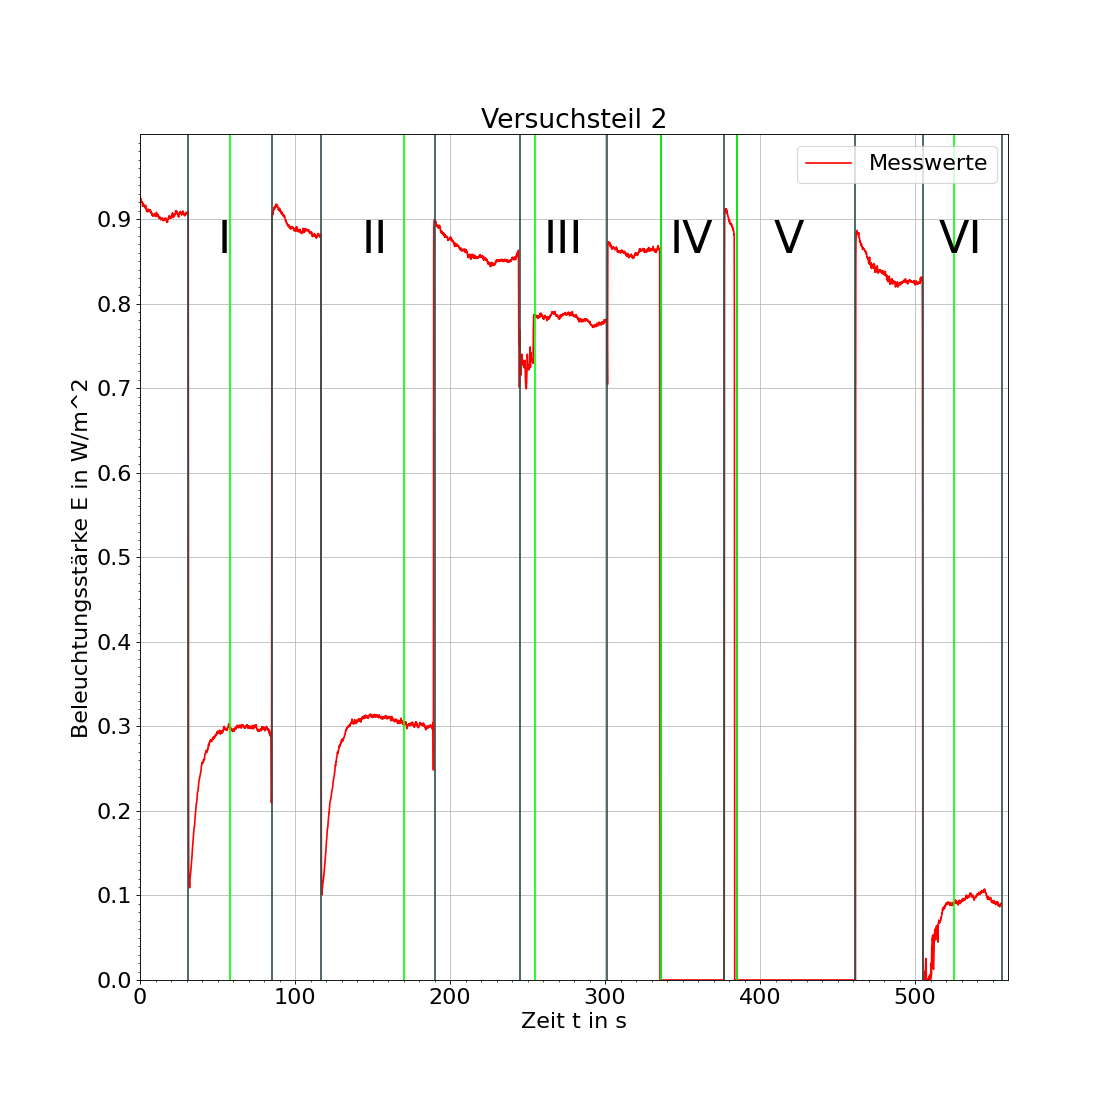
\includegraphics[width=0.9\textwidth]{Daten/Matplot.png}
                \caption{Plot der Messwerte für die verschiedenen Materialien. Die grünen Linien kennzeichnen
                den Beginn des stationären Bereich, die Grauen beranden ein Intervall eines Materials}
            \end{figure}

            Aus diesen Werten ließen sich die Intervalle der verschiedenen Materialien bestimmen
            und in dem jeweiligen Intervall auch der minimale Transmissionswert $I$ und der Durchschnittswert
            im stationären Bereich $I_0$.\\
            Daraus lies sich folgende Tabelle mit den Transmissionswerten $\frac{I}{I_0}$ des jeweiligen Materials
            bestimmen.
            \begin{center}
                \begin{tabular}{|c|c|c|c|c|c|c|}
                    \hline
                    Material & $I_{air}[\frac{W}{m^2}] $ & $I_0[\frac{W}{m^2}]$ & $I[\frac{W}{m^2}]$ & $\frac{I}{I_{air}}[\%]$ & $\frac{I_0}{I_{air}}[\%]$ & $\frac{I}{I_0}[\%]$\\
                    \hline
                    I - Lila Farbfolie              & $0,906\pm 0,09$ & $0,297\pm 0,03$     & 0,109 & $12,03\pm 0,10$ & $32,82\pm 0,04$ & $36,74\pm 0,12$ \\
                    II - Orange Farbfolie           & $0,889\pm 0,12$ & $0,317\pm 0,03$     & 0,101 & $11,36\pm 0,24$ & $35,66\pm 0,07$ & $31,65\pm 0,11$ \\
                    III - Transparente Farbfolie    & $0,860\pm 0,18$ & $0,783\pm 0,10$     & 0,700 & $81,40\pm 0,44$ & $91,04\pm 0,34$ & $89,35\pm 0,14$ \\
                    IV - Blatt Papier               & $0,859\pm 0,09$ & $0,001\pm 0$        & 0     & $<0,01\pm 0$ & $0\pm 0 $     & $0\pm 0$     \\
                    V - Taschentuch                 & $0,888\pm 0,06$ & $<0,001\pm 0$       & 0     & $<0,01\pm 0$ & $0\pm 0 $     & $0\pm 0$     \\
                    VI - Eine Lage Taschentuch      & $0,733\pm 0,11$ & $0,096\pm 0,08$     & 0,005 & $<0,01\pm 0$ & $13,10\pm 0,10$ & $4,25\pm 0,90$  \\
                    \hline
                \end{tabular}
            \end{center}
            Es ist deutlich zu erkennen das verschiedene Materialien die IR-Strahlung verschieden
            gut Absorbieren. So absorbieren die Farbfolie zwischen 60\% und 70\% der IR-Strahlung,
            das Papier und Taschentuch jedoch ~100\%. Diese Unterschiede lassen sich unter anderem
            auf die Farbe des Materials zurückführen, da diese durch das Fehlen des Lichts jener
            Wellenlänge bestimmt wird. IR-Strahlung liegt zwar größtenteils außerhalb des sichtbaren
            Bereichs, jedoch wird bei der Erzeugung häufig auch sichtbares rotes Licht emittiert, welches
            hier von der orangen Folie am besten absorbiert wird. Das Blatt Papier sowie die Variationen
            des Taschentuchs erscheinen Weiß, da sie das gesamte Spektrum absorbieren wie auch an der
            Transmission zu erkennen ist. Es fällt jedoch auf, das bei nur einer Lage des Taschentuchs
            noch ein wenig Strahlung durch zu kommen scheint, dieser Effekt ist wahrscheinlich auf die
            %Tunneleffekt zurück zu führen, bei dem einige wenige Photonen nicht absorbiert oder reflektiert werden sonder Tunneln, wobei bei besonders dünnen Schichten die Wahrscheinlichkeit eines solchen Phänomens höher ist
            Struktur des Papiers zurück zu führen. Für eine derart kleine Wellenlänge besitzt eine Lage Papier, insbesondere
            so dünnes Papier wie einlagiges Taschentuchpapier, Löcher durch die die Strahlung zum Detektor gelangt.
            Die Wahrscheinlichkeit ein solches Loch zu treffen
            nimmt mit jeder zusätzlichen Lage ab, da dort 2 Löcher überlappen müssten um noch
            Strahlung durch zu lassen. Zuletzt betrachten wir die Transparente Folie, die so gut wie keine Strahlung absorbiert,
            jedoch ist der Wirkungsquerschnitt des Materials nicht gleich 0 sodass es dennoch in seltenen 
            Fällen zu Reflektion oder Absorption kommen kann.\\
            Bei den meisten Materialien sieht man zusätzlich noch einen exponentiellen Anstieg der Beleuchtungsstärke mit 
            der Zeit. Diese Veränderung entsteht durch die Erwärmung des Materials durch die sich die Materialien ein klein wenig
            ausdehnen und so einen geringeren Wirkungsquerschnitt aufweisen wodurch mehr Strahlung transmittiert wird. Auch beginnen die Materialien durch die Erwärmung selber zu emittieren.
             
        \subsection{IR-Absorption in $CO_2$ bei bekannter Konzentration}
            Nun wollen wir unsere bisherigen Überlegungen auf die $CO_2$ Konzentration in unserem Gasbehälter
            anwenden. Dazu wird eine bekannte Menge $CO_2$ in das bekannte Volumen injiziert, woraus
            die Konzentration in dem Volumen folgt:
            \begin{equation}
                V_{zylinder} = \pi r^2 x = \pi (\frac{3,93}{2} cm)^2 *15cm = 181,96ml
            \end{equation}
            \begin{equation}
                Konzentration = V_{CO_2}/V_{zylinder}
            \end{equation}
            Passend zu den Konzentrationen lässt sich aus den Messdaten die Leuchtstärke
            ohne $CO_2$ $I_0$ und mit $CO_2$ I bestimmen.
            
            
            \begin{figure}[H]
                \centering
                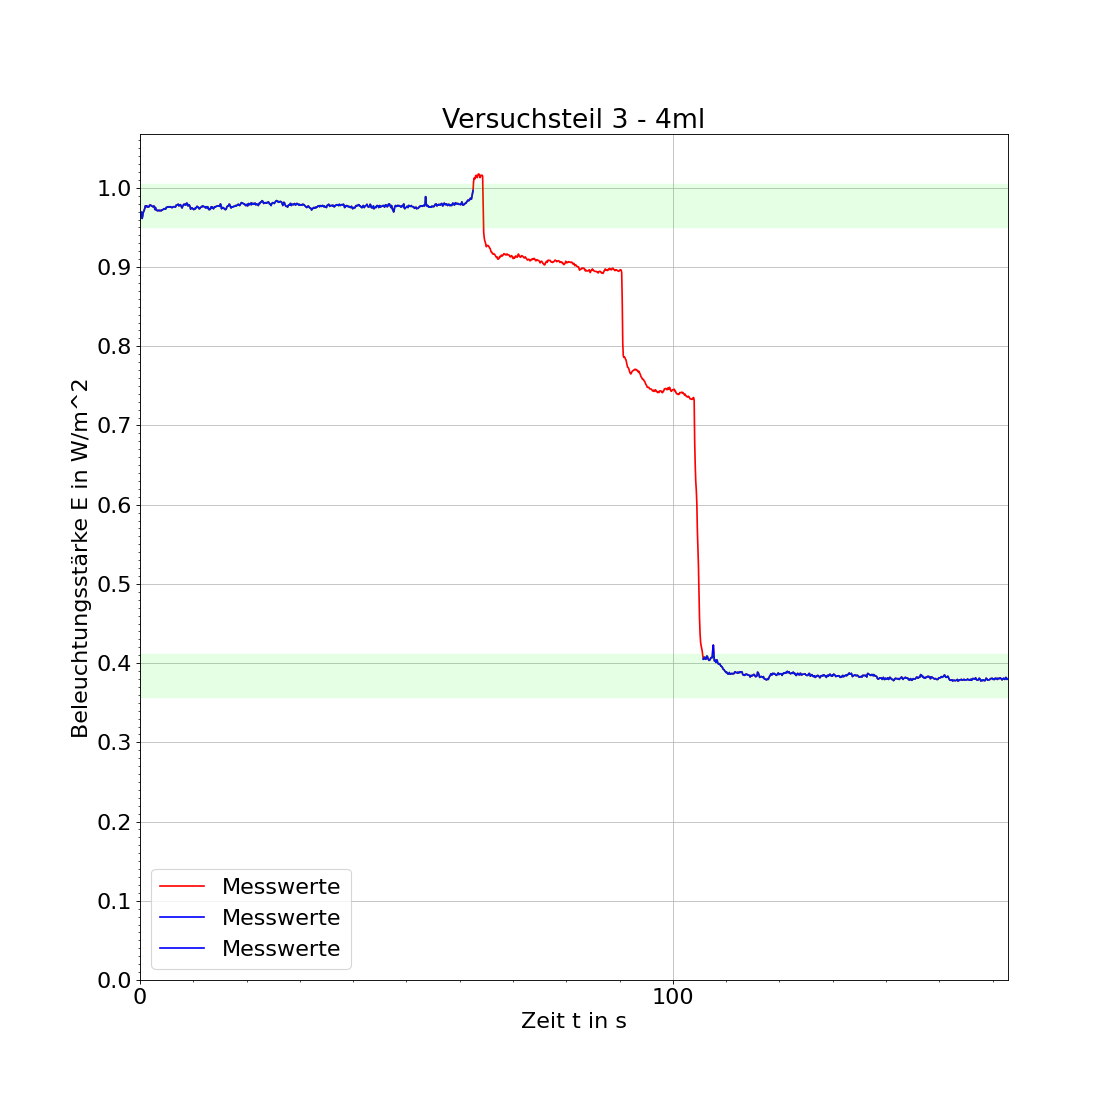
\includegraphics[width=0.9\textwidth]{Daten/KonzPlot4ml.png}
                \caption{Bestimmung von I und $I_0$ anhand der Messdaten}
            \end{figure}
            \hspace{1cm}
            \begin{center}
                \begin{tabular}{|c|c|c|c|c|}
                    \hline
                    $CO_2$ [ml] & Konzentration [\%] & $I [W/m^2]$ & $I_0 [W/m^2]$ & $\frac{I}{I_0}$ \\
                    \hline
                    0      & 0     & $0,897\pm 0,07$& $0,897\pm 0,070$& $1\pm 0.078$\\
                    2      & 1,1   & $0,543\pm 0,23$& $0,982\pm 0,095$& $0,553\pm 0,238$\\
                    3      & 1,649 & $0,528\pm 0,19$& $0,977\pm 0,039$& $0,540\pm 0,192$\\
                    4      & 2,198 & $0,384\pm 0,15$& $0,977\pm 0,076$& $0,393\pm 0,154$\\
                    5      & 2,748 & $0,433\pm 0,14$& $0,902\pm 0,126$& $0,479\pm 0,167$\\
                    10     & 5,496 & $0,217\pm 0,14$& $0,920\pm 0,147$& $0,236\pm 0,161$\\
                    15     & 8,244 & $0,185\pm 0,14$& $0,909\pm 0,020$& $0,203\pm 0,160$\\
                    20     & 10,992 & $0,162\pm 0,13$& $0,901\pm 0,163$& $0,180\pm 0,142$\\
                    30     & 16,488 & $0,115\pm 0,10$& $0,850\pm 0,063$& $0,135\pm 0,118$\\
                    45     & 24,731 & $0,087\pm 0,08$& $0,882\pm 0,174$& $0,099\pm 0,094$\\
                    60     & 32,975 & $0,045\pm 0,24$& $0,881\pm 0,094$& $0,051\pm 0,268$\\
                    181    & 99,474 & $0,003\pm 0,09$& $0,879\pm 0,094$& $0,003\pm 0,097$\\
                    \hline 
                \end{tabular}
            \end{center}
            Nun lässt sich für die verschiedenen Konzentrationen die Lambert-Beer-Gaußkurve
            bestimmen über:
            \begin{equation}
                \begin{aligned}
                    &g_s(\nu) = \frac{I(\nu)}{I_0} = exp(-Cx\beta exp(-\frac{(\nu-\nu_0)^2}{2\sigma^2}))\\
                    &\sigma = 1\\
                    &\nu_0 = 0\\
                    &\nu \in [-10,10]\\
                    &C = Konzentration \\
                    &\beta x = freier Parameter
                \end{aligned}
            \end{equation}
            \begin{figure}[H]
                \centering
                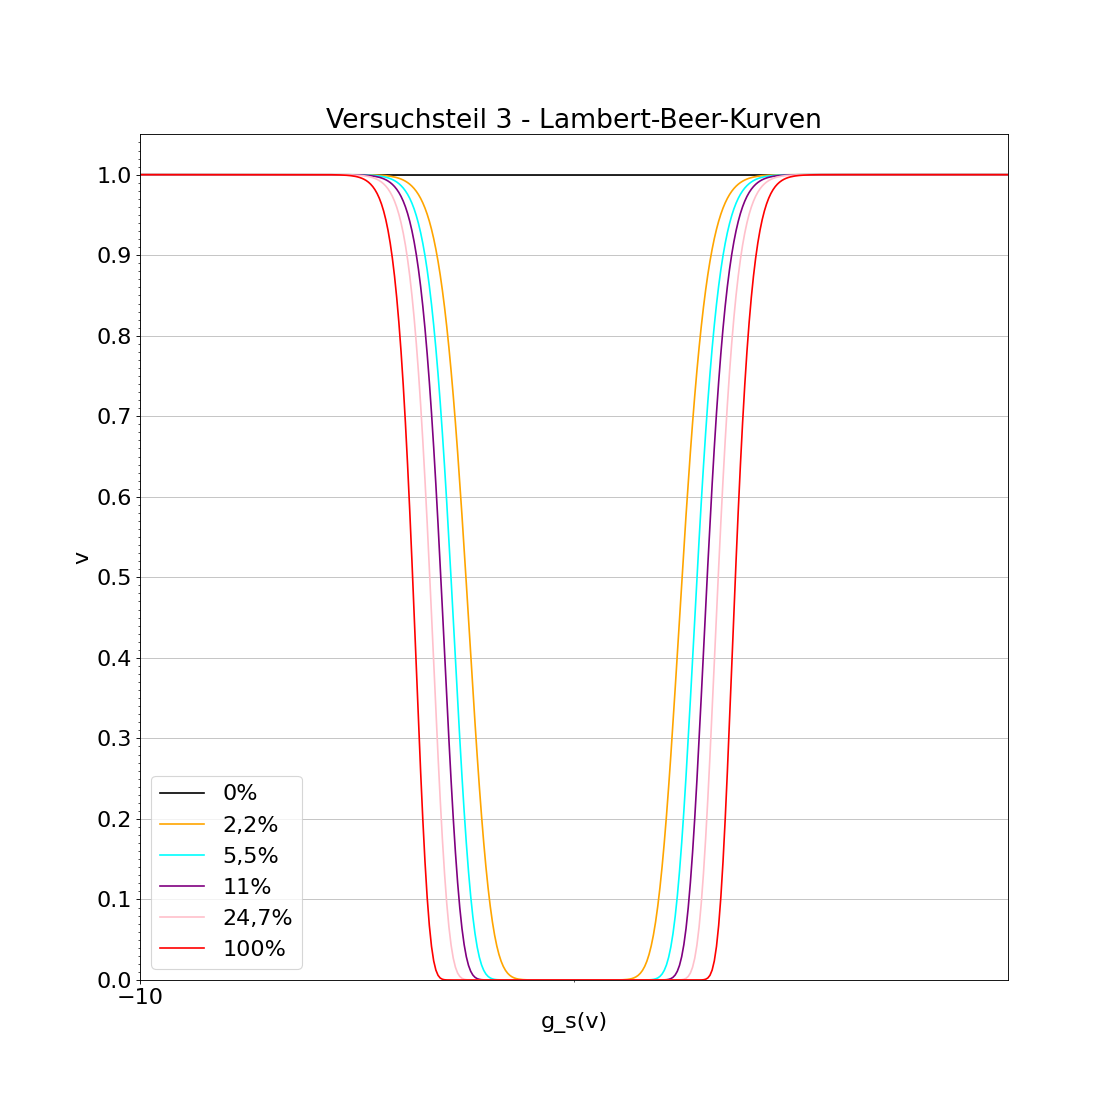
\includegraphics[width=0.7\textwidth]{Daten/LambertBeer.png}
                \caption{Lambert-Beer-Kurven für eine Auswahl an Konzentrationen mit $\beta$x = 7}
            \end{figure}

            Diese Funktionen lassen sich für jede Konzentration numerisch von $\nu \in [-10,10]$
            integrieren.
            \begin{equation}
                T(C) = h \cdot \sum_{n} g_s(\nu_n)
            \end{equation}
            wobei hier h = 0.05 ist.\\
            Aus den Transmissionen T(C) lässt sich über
            \begin{equation}
                T_{rel}(C) = \frac{T(C)-T(100\%)}{T(0\%)-T(100\%)}
            \end{equation}
            die relative Transmission bestimmen. Diese muss nun noch um einen Faktor
            und einen Offset korrigiert werden, da auch bei einer 100\% $CO_2$ Konzentration
            noch eine Beleuchtungsstärke zu messen ist durch die breitere Detektorcharakteristik.
            Um nach der Offset Korrektur dennoch eine Deckung mit den Messwerten zu erreichen
            Werden die Werte um einen Faktor skaliert.
            \begin{equation}
                \begin{aligned}
                    Offset = T_{rel}(100\%)\\
                    Faktor = 1-Offset
                \end{aligned}
            \end{equation}
            Um nun eine möglichst genaue Deckung mit den Messwerte zu erzielen muss der
            Faktor $\beta x $ variiert werden.
            \begin{figure}[H]
                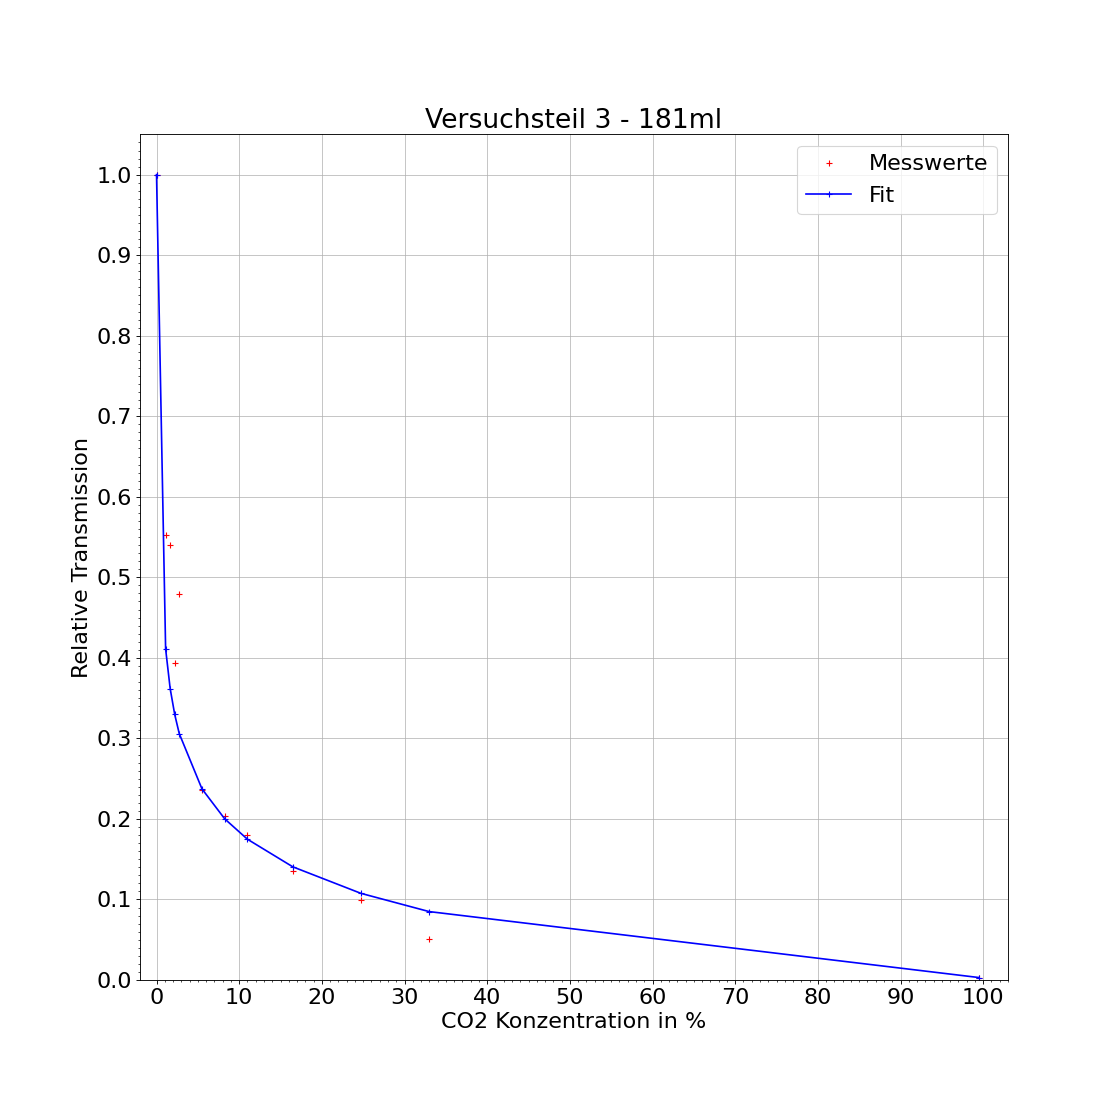
\includegraphics[width=0.9\textwidth]{Daten/KonzPlot.png}
                \caption{Fit der Lamber-Beer Funktionen an die Messwerte} 
            \end{figure}
            Daraus folgt hier
            \begin{equation}
                \begin{aligned}
                    \text{Offset} = 0,003\\
                    \text{Faktor} = 1-0,003\\
                    \beta x = 7
                \end{aligned}    
            \end{equation}
            Aus Abbildung 8 folgt, das die Empfindlichkeit des Detektors bei 
            niedrigen Konzentrationen von $CO_2$ deutlich höher ist, als bei hohen Konzentrationen.
            Dies ist daran zu erkennen, das sich bei niedrigen Konzentrationen selbst bei Änderungen
            von wenigen Milliliter eine verhältnismäßig starke Änderung der relativen Transmission zu erkennen ist,
            wohingegen bei hohen Konzentrationen wenige Milliliter nur schwer von einander zu Unterscheiden sind.\\
            Um die minimale Konzentration die mit einer Genauigkeit von 10\% zu bestimmen ist zu ermitteln,
            ist zunächst der Fehler für $I_0$ ab zu schätzen, dafür bestimmt man den Mittelwert der $I_0$ und deren
            Standardabweichung
            \begin{equation}
                \begin{aligned}
                    \overline{I_0} = 0,913 [\frac{W}{m^2}]\\
                    \Delta \overline{I_0} = 0.0017 [\frac{W}{m^2}]
                \end{aligned}
            \end{equation}
            Die Transmissionsmessung hat eine Unsicherheit von
            10\%, wenn die Differenz von I und $I_0$ das zehnfache des Fehlers betragen, also wenn folgendes gilt:
            \begin{equation}
                \overline{I_0} - I = 10 \Delta \overline{I_0} \Leftrightarrow I = \overline{I_0} - 10 \Delta \overline{I_0}
            \end{equation}
            Daraus folgt, dass die minimal mit $CO_2$ bestimmbare Intensität $I = 0,896 [\frac{W}{m^2}]$ ist.
            Das entspricht einem Transmissionswert von 
            \begin{equation}
                \frac{I}{\overline{I_0}} = 0,981
            \end{equation}
            Was einer Konzentration von etwa $(0,008\pm0,001)\% = 125ppm$ entspricht.
            Da die durchschnittliche Raumluft einen $CO_2$ Gehalt von etwa 0,04\% hat,
            lässt sich diese zuverlässig mit diesem Spektrometer bestimmen.
            
            \begin{center}
             
            \end{center}
            

            Das verwendete Modell stellt sich als realistisch heraus. Zwei getroffene Annahmen könnten jedoch zu einem Fehler führen:
            \begin{itemize}
            	\item Der Wendel wurde als schwarz Körper angenommen, obwohl er keiner ist
            	\item Es ist möglich, dass bei der Zufuhr von $CO_2$ das Gas teilweise entweicht
            \end{itemize}
            
            Bei Bestimmung des $CO_2$-Anteils in der Luft sollte man außerdem berücksichtigen, dass es in der Luft auch Verunreinigungen, wie z.B. andere IR-Aktive Treibhausgase gibt. 
            Sowie mögliche Unterschiede in der Lufttemperatur.
            Auch ist die Elektronik nicht perfekt, so dass Ungenauigkeiten und Schwankungen auftreten könnten.
            \subsection{Messung der $CO_2$-Konzentration in der Luft durch IR-Absorption}
            Nun lässt sich die bestimmte Kalibrationskurve anwenden um den $CO_2$ Gehalt der
            Raumluft zu bestimmen. Dazu wird der Zylinder belüftet und die Intensität gemessen.
            Danach lässt sich durch das Variieren bzw. fitten von C zu gegebener Transmission
            \begin{equation}
                \begin{aligned}
                    \text{Intensität ohne $CO_2$ } I_0 = (0,956\pm0,121)W/m^2 \\
                    \text{Intensität mit Raumluft } I = (0,764\pm0,062)W/m^2 \\  
                    \text{Transmission } \frac{I}{I_0} = 0,797 \\
                    \Delta \frac{I}{I_0} = \sqrt{(\frac{\Delta I}{I_0})^2 + (\frac{\Delta I_0 \cdot I}{I_0^2})^2} = 0,12
                \end{aligned}
            \end{equation} 
            die Konzentration C in \% bestimmen. In der gemessenen Raumluft ergab sich dadurch eine
            Konzentration von etwa 0,115\% bzw. 1150ppm. Dieser Wert liegt jedoch weit über dem Durchschnitt 
            von etwa 0,04\% bzw. 400ppm.
            \begin{figure}[H]
                \centering
                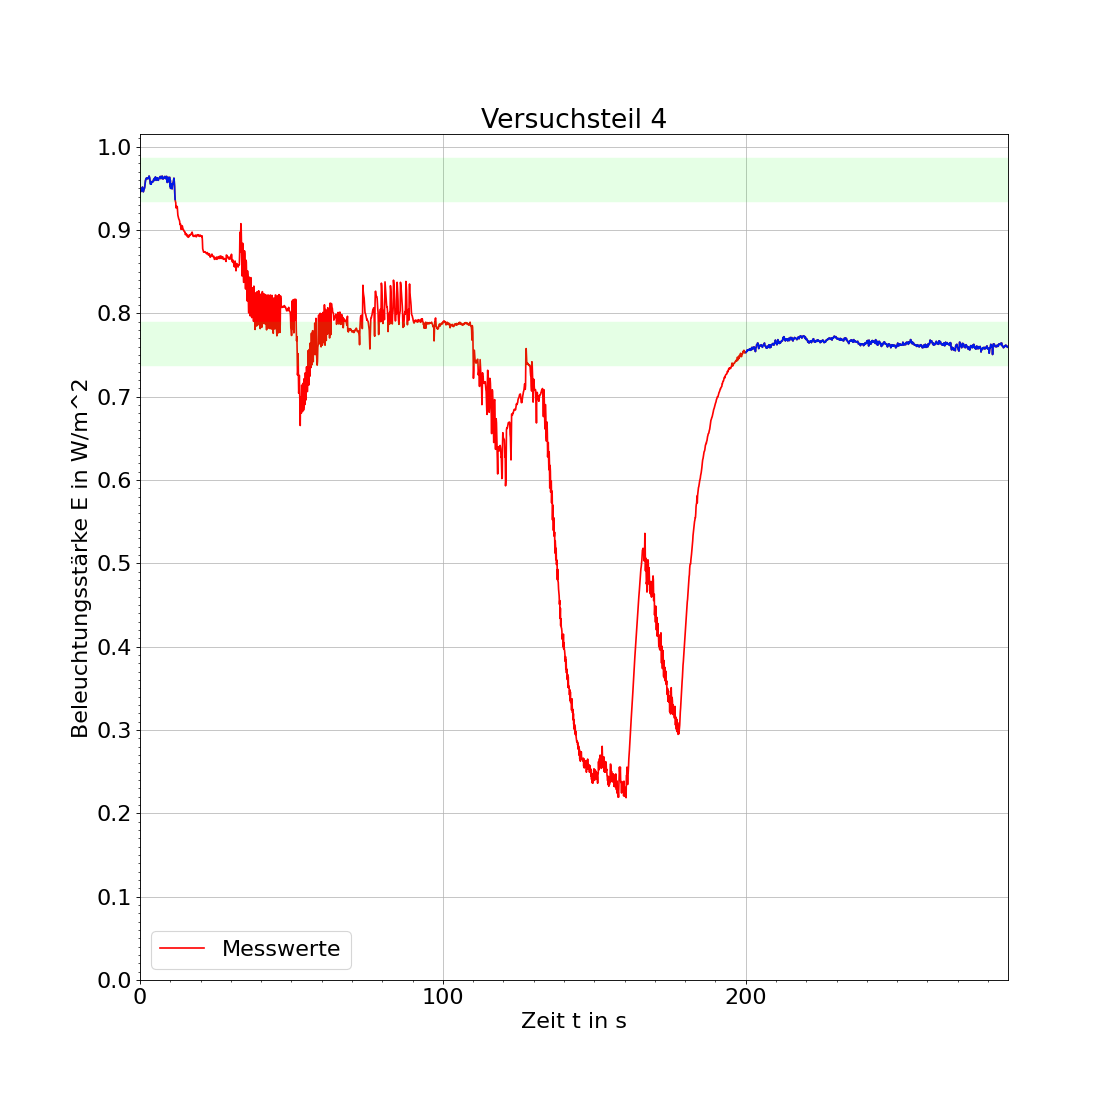
\includegraphics[width=0.8\textwidth]{Daten/LuftPlot.png}
                \caption{Messung der Raumluft, die blau markierten Bereiche kennzeichnen I und $I_0$}
            \end{figure}

            \subsection{Zusatzversuch}
                Bei der Beobachtung der Glühwendel ergab sich für den Stromwert bei der
                das rote Glühen erstmals zu erkennen war $I = 4,6A$.
                Daraus folgt eine Temperatur von 
                \begin{equation}
                    T[K] = 79\frac{K}{A}\cdot I +202K = 565,4K 
                \end{equation}
                für die Glühwendel.\\
        \section{Diskussion} 
            Der Versuch schien weitgehend erfolgreich, da sich der exponentielle Zusammenhang von
            $CO_2$ Konzentration und Transmissivität gut bestätigen lies, und die daraus folgende
            Kalibrationskurve eine sehr hohe Auflösung versprach. Hier lässt sich jedoch ein Fehler vermuten,
            da eine derart hohe Messgenauigkeit mit einem solchen Aufbau nur schwer nach zu vollziehen
            ist, aufgrund der Vielzahl an Störfaktoren und Varianzen, sowie beispielsweise die 
            Strahlungsleistung der Wendel oder diverse Temperatur bedingte Änderungen, der Einfluss
            der Verwirbelung der Raum- bzw. Umgebungsluft auf die selbige. Dieser Verdacht eines Fehlers
            verstärkt sich durch Versuchsteil 4, bei dem die Bestimmung der $CO_2$ Konzentration der Raumluft
            etwa 1.150ppm ergab, obwohl der durchschnittliche Literaturwert nur bei etwas einem Drittel davon
            liegt (etwa 400ppm). Hier könnte eine Verunreinigung der Luft im Zylinder vorgelegen haben,
            oder ein Luftzug im Zylinder durch die Öffnung des Systems. Jedoch sollte auch in Betracht
            gezogen werden, das bei der Kalibrationskurve ein Fehler aufgetreten ist, den wir jedoch nicht
            näher ermitteln konnten.
\end{document}